\part{Circuito de Aplicación: Sensor de Temperatura}
En esta parte del presente trabajo, se pidió implementar un circuito que adapte la señal de un sensor de temperatura \emph{LM35}. Se solicitó que la señal de salida del circuito diseñado fuera apropiada para ser adquirida por un sistema con tensión de entrada variable entre $0V$ y $5V$.

\section{Diseño del Circuito}
Como condición de diseño, se pidió que el circuito adapte las señales correspondientes a temperaturas que varían entre $35^\circ$ y $45^\circ$ en un rango de tensiones de salida comprendidas entre $0V$ y $5V$ ($35^\circ C \rightarrow 0V$ ; $45^\circ C \rightarrow 5V$).

\subsection{LM35}
Como primer paso se inspeccionó la hoja de datos del sensor que se utilizó en el diseño. Los parámetros relevantes que se extrajeron de la misma fueron la tensión de alimentación, y la tensión de salida en función de la temperatura. 

Respecto a la alimentación, el sensor admite tensiones de alimentación comprendidas entre $+4V$ y $+20V$, la cual se proporciona entre un terminal \emph{Vs} y \emph{GND}. Respecto a la tensión de salida (proporcional a la temperatura del sensor), la misma está dada por la siguiente expresión:

\[V_{T}(T) = 0mV + 10.0mV / ^\circ C * T\]

Donde la temperatura \emph{T} esta en $^\circ C$. Utilizando esta información se determinaron las tensiones correspondientes las temperaturas de $35^\circ C$ y $45^\circ C$:

\[V_T(35^\circ C) = 350mV\]
\[V_T(45^\circ C) = 450mV\]

De esta forma, se puede establecer una relación entre la tensión proporcionada por el sensor y la tensión de salida esperada (impuesta por la condición de diseño comentada al comienzo del apartado):

\[V_T = 350mV \rightarrow V_{out} = 0V\]
\[V_T = 450mV \rightarrow V_{out} = 5V\]

\subsection{Linealidad de la salida: Implementación con amplificadores operacionales}\label{linealidad}
Se estableció que la tensión de salida $V_{out}$ correspondería a una función lineal dependiente de la tensión de entrada $V_T$ (generada por el sensor). Para lograr este resultado se propuso la siguiente expresión de \emph{Vout} en función de \emph{Vin}:

\begin{equation}
\label{expresion_lineal}
V_{out}(V_{in}) = k V_{in} + V_2
\end{equation}


Dadas las siguientes condiciones iniciales, impuestas como regla de diseño:

\[V_{out}(0.350V) = k(0.350V) + V_2 = 0V\]
\[V_{out}(0.450V) = k(0.450V) + V_2 = 5V\]

Despejano, se obtiene:

\begin{equation}
\label{valor_k}
k = 50
\end{equation}
\begin{equation}
\label{valor_V2}
V_2 = -17.5V
\end{equation}



\subsubsection{Dagrama de señal y cálculo de parámetros}
Se procedió a trazar un diagrama de señal que me permitiera obtener la expresión deseada, a partir de módulos amplificadores y sumadores (que se pueden implementar con amplificadores operacionales). El diagrama resultante fue:

\begin{figure}[H]
\centering
\begin{circuitikz}

	\node [label=left:$v_{in}$](Vin) at (0,0){};
	\node [right = 3cm of Vin](V2){};
	\node [label=left:$V_{off}$,below = 2cm of V2](Voff){};
	\node [right = 3cm of V2](V3){};
	\node [below = 2cm of V3](V4){};
	\node [adder](sum) at ($(V3)!0.5!(V4)$){};
	\node [mixer,label={[label distance=0.5cm]270:$-1$},right = 1cm of sum](mix){};
	\node [right = 1cm of mix,label=right:$v_{out}$](Vout){};
	
	
	\draw (Vin) to[twoport,t=$-k_1$,o-o] (V2);
	\draw (V2) to[twoport,t=$k_A$,o-] (V3);
	\draw (Voff) to[twoport,t=$k_B$,o-] (V4);
	
	\draw (V3) to[short] (sum.4);
	\draw (sum.4) node[inputarrow,rotate=270]{};
	
	\draw (V4) to[short] (sum.2);
	\draw (sum.2) node[inputarrow,rotate=90]{};
	
	\draw (sum.3) to[short] (mix.1);
	\draw (mix.1) node[inputarrow]{};	
	
	\draw (mix.3) to[short,-o] (Vout);
\end{circuitikz}
\caption{Diagrama de señal del circuito a implementar}
\label{6_signal_diagram}
\end{figure}

Si se calcula la señal $v_{out}$ en función de $v_{in}$, considerando que los demas parámetros del diagrama son valores constantes, se obtiene:

\begin{equation}
\label{salida_flujo}
v_{out} = (k_1 k_A) v_{in} + (-k_B V_{off})
\end{equation}

Al analizar la expresión \ref{expresion_lineal} se pudo establecer una equivalencia entre el factor $k$ y $(k_1 k_A)$, y entre el término $V_2$ y $(-k_B V_{off})$ para obtener la salida deseada utilizando el diagrama de señal de la Figura \ref{6_signal_diagram}, entonces, se estableció que:

\begin{equation}
\label{k_igualdad}
k = k_1 k_A = 50;
\end{equation}
\begin{equation}
\label{V2_igualdad}
V2 = -k_B V_off = -17.5V
\end{equation}

Habiendo establecido valores para los módulos de la Figura \ref{6_signal_diagram}, el problema se trasladó a implementar el diagrama mediante dos amplificadores operacionales. Las dos fases en cascada a implementar se muestran en las Figuras \ref{6_f1} y \ref{6_f2}.

\begin{figure}[H]
\centering
\begin{circuitikz}

	\node [label=left:$v_{in}$](Vin) at (0,0){};
	\node [right = 3cm of Vin,label=right:$-k_1 v_{in}$](V2){};
	
	\draw (Vin) to[twoport,t=$-k_1$,o-o] (V2);

\end{circuitikz}
\caption{Primera fase del diseño: Amplificador inversor}
\label{6_f1}
\end{figure}

\begin{figure}[H]
\centering
\begin{circuitikz}

	\node [label=left:$-k_1 v_{in}$](V2) at (0,0){};
	\node [label=left:$V_{off}$,below = 2cm of V2](Voff){};
	\node [right = 3cm of V2](V3){};
	\node [below = 2cm of V3](V4){};
	\node [adder](sum) at ($(V3)!0.5!(V4)$){};
	\node [mixer,label={[label distance=0.5cm]270:$-1$},right = 1cm of sum](mix){};
	\node [right = 1cm of mix,label=right:$-(k_A (-k_1 v_{in}) + k_B (V_{off}))$](Vout){};
	
	
	\draw (V2) to[twoport,t=$k_A$,o-] (V3);
	\draw (Voff) to[twoport,t=$k_B$,o-] (V4);
	
	\draw (V3) to[short] (sum.4);
	\draw (sum.4) node[inputarrow,rotate=270]{};
	
	\draw (V4) to[short] (sum.2);
	\draw (sum.2) node[inputarrow,rotate=90]{};
	
	\draw (sum.3) to[short] (mix.1);
	\draw (mix.1) node[inputarrow]{};	
	
	\draw (mix.3) to[short,-o] (Vout);
\end{circuitikz}
\caption{Segunda fase del diseño: Amplificador sumador}
\label{6_f2}
\end{figure}




\subsubsection{Primera Fase: Amplificador Inversor}
La Figura \ref{6_invert_opamp_fig} muestra un amplificador operacional configurado en modo inversor. La transferencia del para una tension continua, se obtiene como:

\[\frac{V_{out}}{V_{in}} = - \frac{R_f}{R_i}\]

y produce una salida

\[V_{out} = -\frac{R_f}{R_1} V_{in}\]

\begin{figure}[H]
\centering
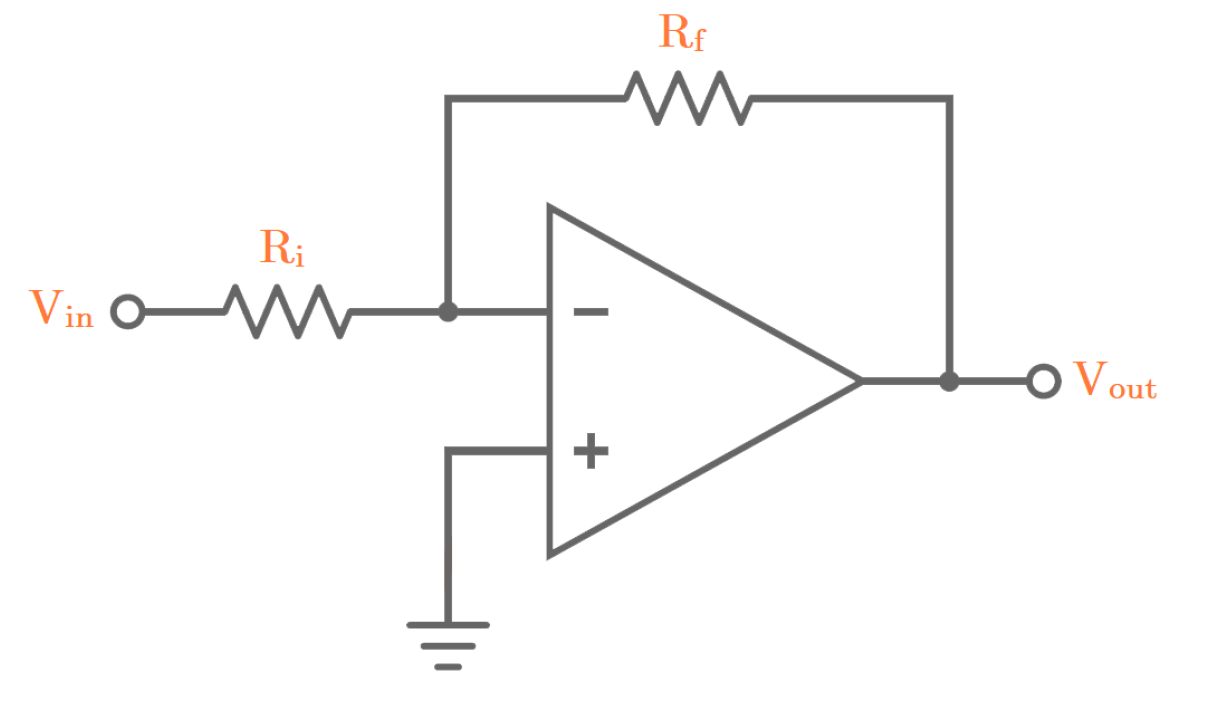
\includegraphics[scale=0.3]{../parte6/Informe/resources/inverting_opamp_diagram.png}
\caption{Circuito amplificador inversor}
\label{6_invert_opamp_fig}
\end{figure}

Para implementar la fase 1, se requiere la siguiente igualdad:

\[-\frac{R_f}{R_1} = - k_1\]

Entonces

\[k_1 = \frac{R_f}{R_1}\]

A partir de esta igualdad ya se pueden establecer valores de las resistencias que implementan el circuito amplificador inversor, cuya elección se detallará mas adelante.

\subsubsection{Segunda Fase: Sumador Ponderado Inversor}
A continuación, en la Figura \ref{6_adder_opamp_fig} se muestra la configuración de un amplificador operacional como sumador ponderado:

\begin{figure}[H]
\centering
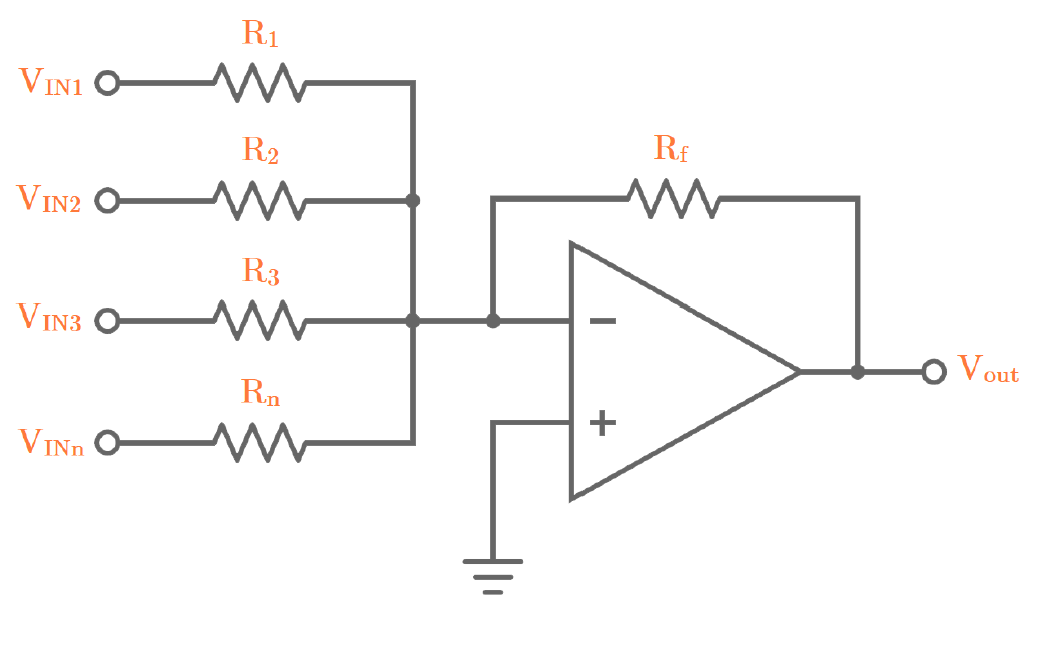
\includegraphics[scale=0.4]{../parte6/Informe/resources/adder_opamp_diagram.png}
\caption{Circuito amplificador sumador ponderado}
\label{6_adder_opamp_fig}
\end{figure}

La salida que produce el circuito es la siguiente:

\[V_{out} = - \left(\frac{R_f}{R_1} V_{IN1} + \frac{R_f}{R_2} V_{IN2} + ... + \frac{R_f}{R_n} V_{INn} \right)\]

A partir de la salida del circuito sumador, y el diagrama de señal de la figura \ref{6_f2} se establecen la siguientes igualdades:

\[k_A = \frac{R_f}{R_1}\]
\[k_B = \frac{R_f}{R_2}\]

\subsection{Fases amplificadoras en cascada}

Explicado el diseño de las dos fases que componen el circuito adaptador de la señal, a continuación se muestra en la Figura \ref{6_amp_2fases} se muestra el circuito que implementa el diseño:

\begin{figure}[H]
\centering
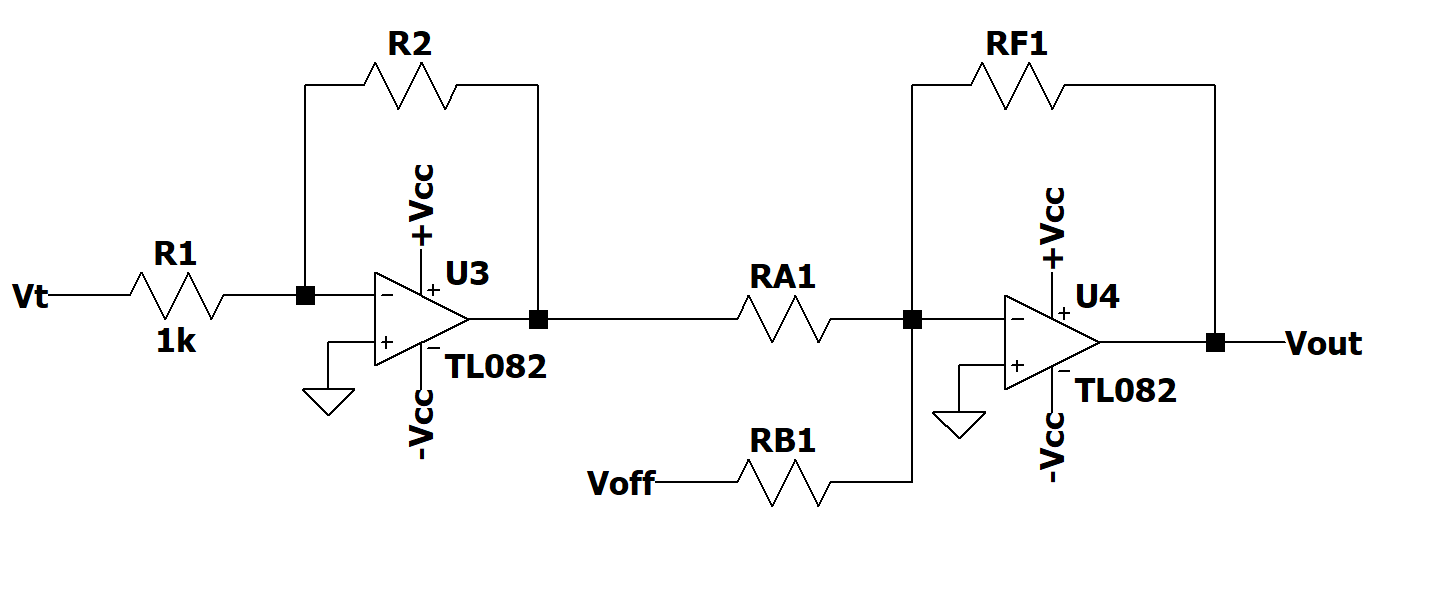
\includegraphics[scale=0.4]{../parte6/Informe/resources/esquematico_opamps.png}
\caption{Circuito que implementa las dos fases de amplificadores operacionales}
\label{6_amp_2fases}
\end{figure}

Siguiendo la nomenclatura de las resistencias de la Figura \ref{6_amp_2fases}, las relaciones entre las resistencias, halladas en los ítemes anteriores son:

\[\frac{R_2}{R_1} = k_1\]
\[ \frac{R_{F1}}{R_{A1}} = k_A\]
\[ \frac{R_{F1}}{R_{B1}} = k_B\]
\[k_1 k_A = 50\]
\[k_B V_{off} = 17.5V\]

Se eligieron los siguientes valores de resistencias y $V_{off}$:

\[R_1 = 1k\Omega\]
\[R_2 = 10k\Omega\]
\[R_{F1} = 10k\Omega\]
\[R_{A1} = 2k\Omega\]
\[R_{B1} = 2k\Omega\]
\[V_{off} = 3.5V\]

La salida analítica esperada del circuito con los valores mencionados se muestra en la Figura \ref{6_analitica}. Curva corresponde a la relación entre tension de salida $V_{out}$ vs. tensión de entrada $V_{in}$. 
Cabe destacar que la gráfica mostrada no contempla la restricción de la limitación de tensión a la salida, la cual se desarrolla en las próximas secciones.

\begin{figure}[H]
\centering
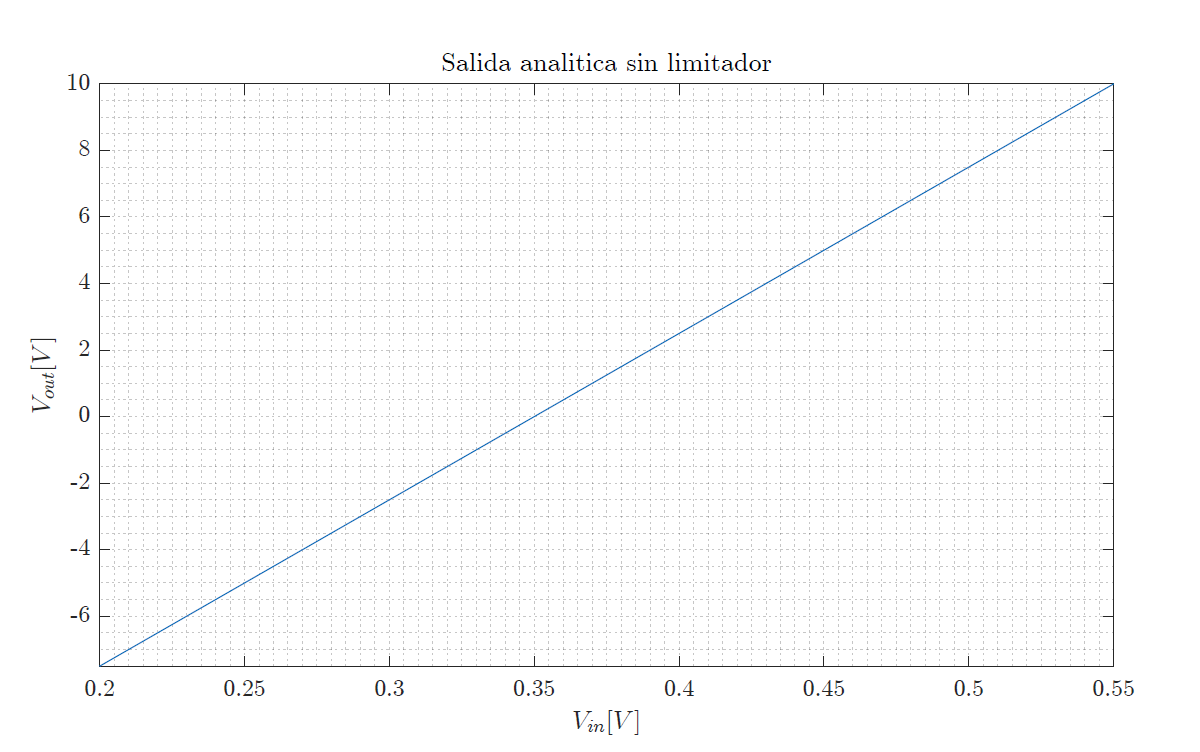
\includegraphics[scale=0.6]{../parte6/Informe/resources/grafica_analitica.png}
\caption{Tensión de salida analítica.}
\label{6_analitica}
\end{figure}

\subsection{Generación de $V_{off}$}

Para generar una tensión de offset $V_{off}$ se implementó un divisor resistivo, como se indica en la Figura \ref{6_v_off}. Mas adelante se detallará la implementación del divisor resistivo mediante una resistencia variable, y su función en la calibración del dispositivo.

\begin{figure}[H]
\centering
\begin{circuitikz}

	\node [label=left:$+V_{cc}$](Vcc) at (0,0){};
	\node [ground, below = 2cm of Vcc](GND){};
	
	\draw (Vcc) to[american potentiometer,n=mypot, o-] (GND);
	\draw (mypot.wiper) to[short,-o] ++(1,0) node[label=right:$V_{off}$](){};
\end{circuitikz}
\caption{Generación de $V_{off}$ con divisor resistivo}
\label{6_v_off}
\end{figure}

\subsection{Limitación de tension de salida}
Se indicaron restricciones respecto a los limites de tensión presentes a la salida del dispositivo. La tensión de salida no debe ser mayor a $+6V$ ni menor a $-1V$. Para lograr esto se dispusieron una serie de diodos a modo de reguladores de tensión. Los mismos se dispusieron como indica la Figura \ref{6_diodos}

\begin{figure}[H]
\centering
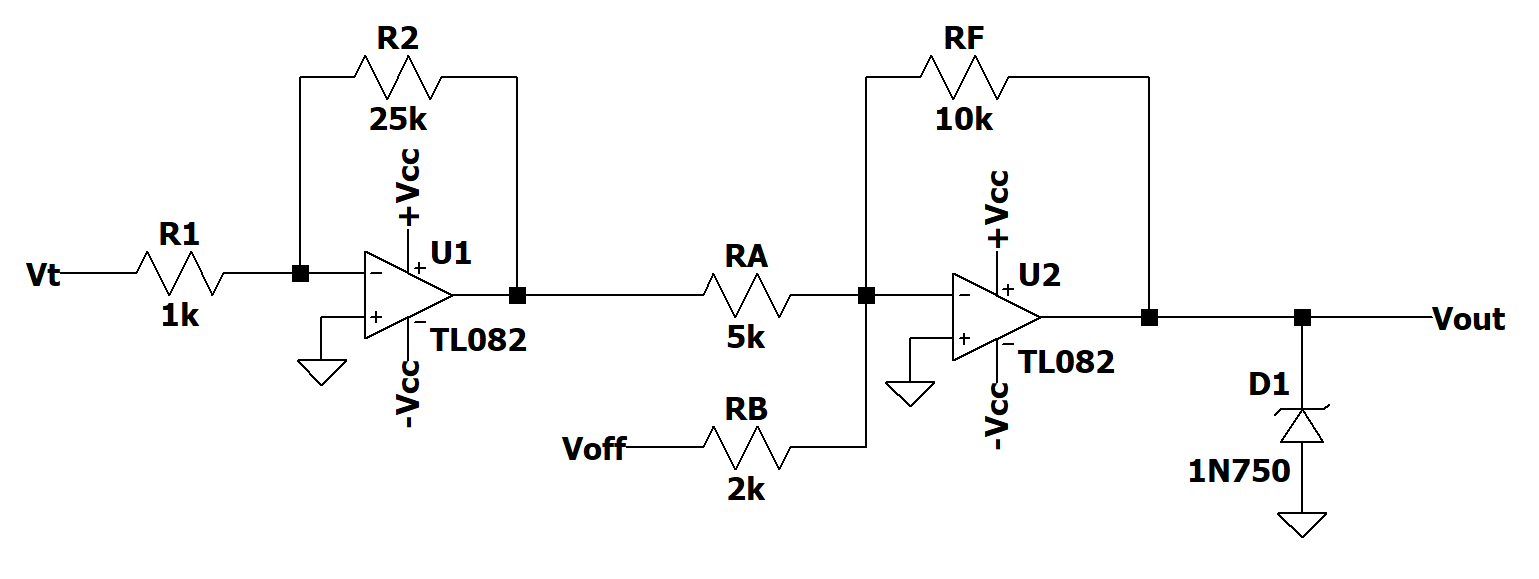
\includegraphics[scale=0.5]{../parte6/Informe/resources/esquematico_opamps_diodos.png}
\caption{Circuito con limitador de tensión}
\label{6_diodos}
\end{figure}

El diodo \emph{D1} limita las tensiones positivas al valore de tensión de ruptura, que ronda los $5,6V$ y las tensiones negativas al valor de su tensión de directa que ronda los $0,7V$. Con esta protección se cumplen los requisitos impuestos.

\section{Simulaciones}
Previo a la implementación fisica del circuito, se llevo a cabo una serie de simulaciones con el objetivo de verificar el funcionamiento del diseño y también determinar la variación de la salida respecto a las tolerancias de las resistencias, de forma tal de elegir el método de calibración adecuado.

\subsubsection{Señal de salida}

\begin{figure}[H]
\centering
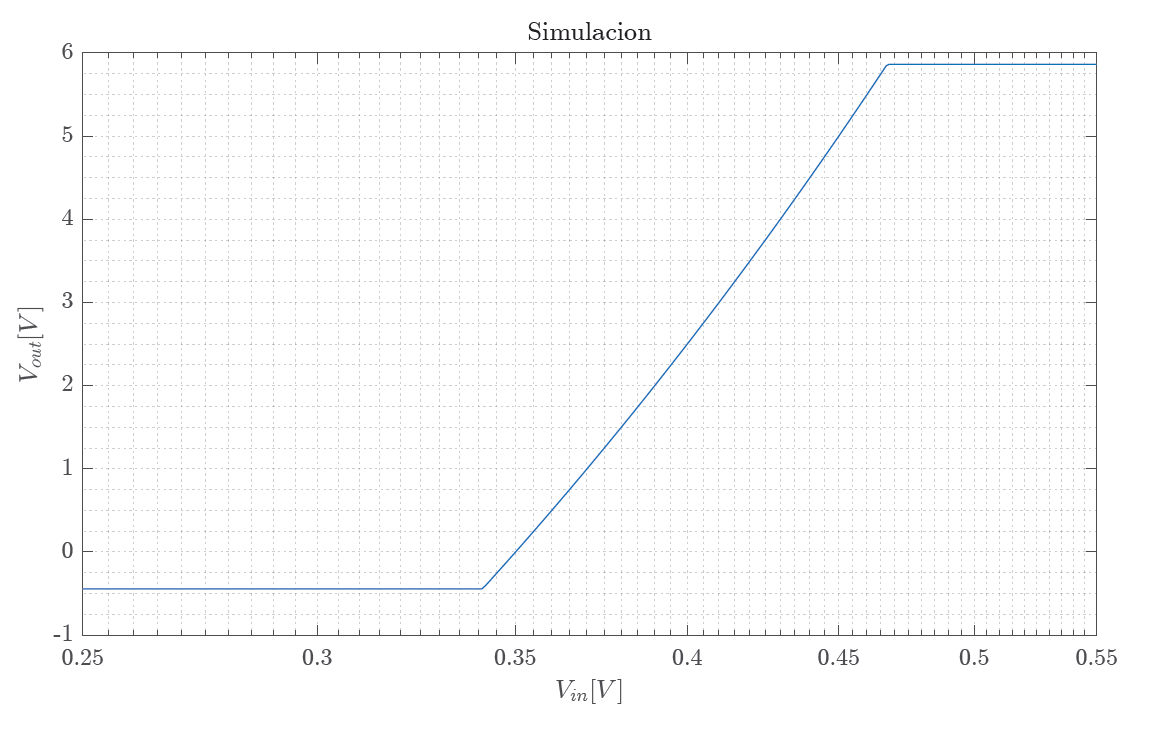
\includegraphics[scale=0.5]{../parte6/Informe/resources/grafica_simulacion.png}
\caption{Circuito simulado en LTspice}
\label{6_simulacion}
\end{figure}

La salida simulada en LTspice se muestra en la Figura \ref{6_simulacion}. Como se observa, le curva se ajusta a la señal analítica presentada en la Figura \ref{6_analitica}, a diferencia que en la simulación están presentes los diodos que limitan la salida.

\subsubsection{Sensibilidades y calibración}

A continuación se realizó un sencillo análisis de sensibilidades para determinar la variación en la señal de salida respecto a los cambios en los valores de las resistencias. Como se determinó en la sección \ref{linealidad}, la señal de salida $V_{out}$ es una recta para el rango de tensiones de entrada comprendido entre $350mV$ y $450mV$, de la forma:

\[V_{out} = k V_{in} + V_2\]

Las deformaciones en la salida pueden estar causadas por variaciones en $k$ o en $V_2$, es decir, sufrirá deformaciones en la pendiente o en el offset.
Las simulaciones de Montecarlo realizadas sobre el circuito mostraron que, excepto $R_F$, todas las resistencias del circuito generaban un corrimiento vertical de la señal de salida, es decir, generaban un offset. Solamente las variaciones de $R_F$ generaron un cambio muy leve en la pendiente.
El efecto mencionado anteriormente se manifiesta en las Figuras \ref{6_mR1}, \ref{6_mRA} y \ref{6_mRF}.

\begin{figure}[H]
\centering
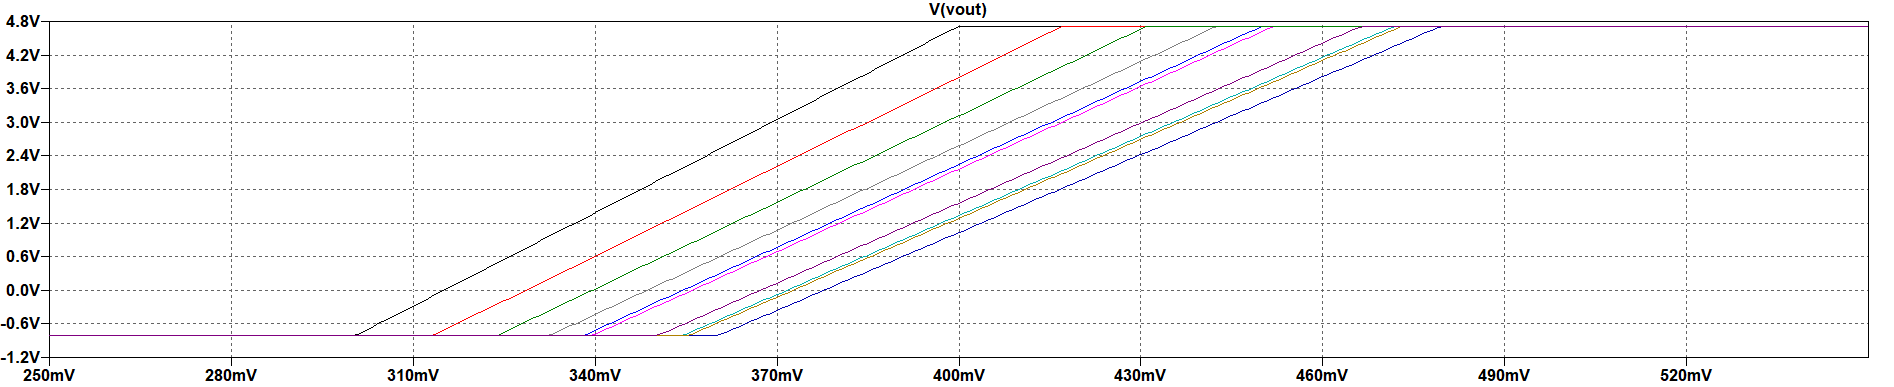
\includegraphics[scale=0.4]{../parte6/Informe/resources/montecarlo_R1.png}
\caption{Variación de la salida variando $R_1$}
\label{6_mR1}
\end{figure}

\begin{figure}[H]
\centering
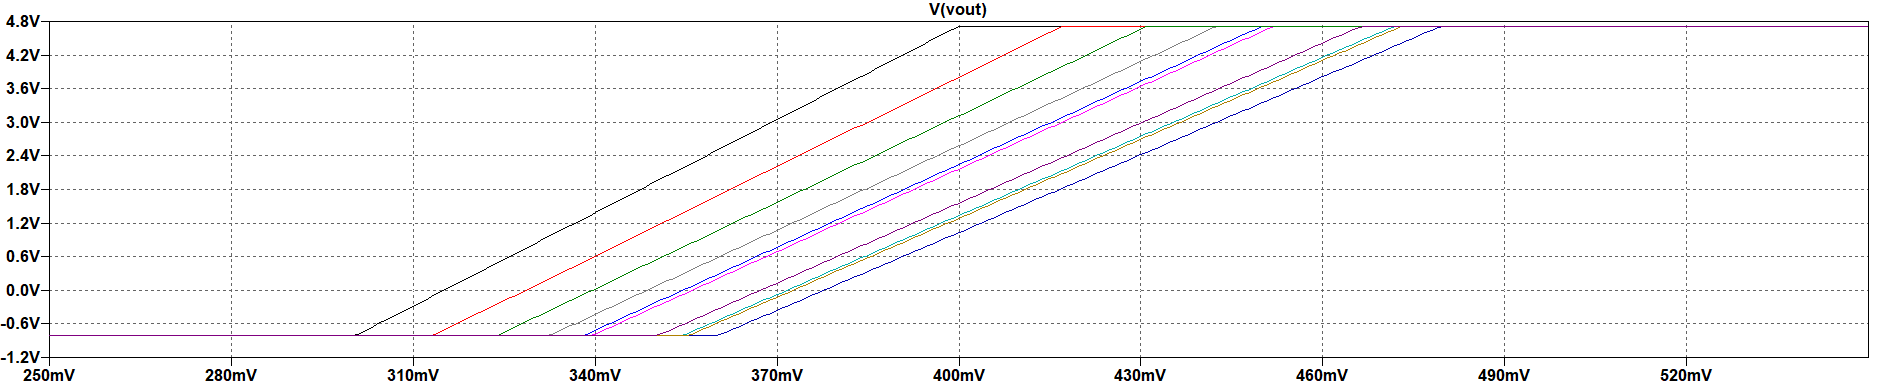
\includegraphics[scale=0.4]{../parte6/Informe/resources/montecarlo_RA.png}
\caption{Variación de la salida variando $R_A$}
\label{6_mRA}
\end{figure}

\begin{figure}[H]
\centering
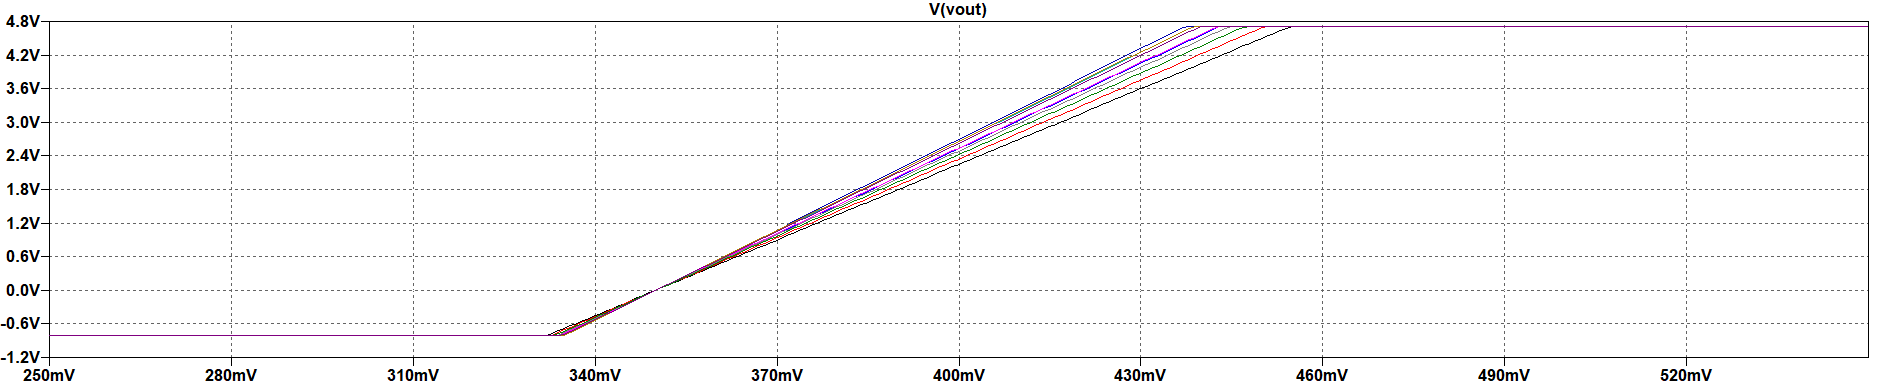
\includegraphics[scale=0.4]{../parte6/Informe/resources/montecarlo_RF.png}
\caption{Variación de la salida variando $R_F$}
\label{6_mRF}
\end{figure}

El hecho de configurar incorrectamente el divisor resistivo que genera la tension $V_{off}$, también genera un corrimiento vertical de la señal de salida.

Habiendo establecido el comportamiento de la salida frente a variaciones en la resistencia, se procedió a determinar el método mas conveniente para la calibración del circuito. Se solicitó que el diseño cuente con solo un dispositivo variable por el usuario para realizar tal calibración. 

Se decidió realizar la calibración por medio del preset que genera la tension $V_{off}$ y la misma se realizara de la siguiente manera. Dado un valor de tensión de entrada $V_{in}$ conocido comprendido entre $350mV$ y $450mV$, se variará $R_{off}$ hasta que el valor de salida sea el esperado


\section{Mediciones}
Se realizaron mediciones sobre la salida del circuito y a la entrada para medir la impedancia de entrada del mismo.

\subsubsection{Señal de salida}
Se alimento el circuito con una fuente de alimentación partido de $\pm 15V$, y se remplazó la señal del integrado LM35 por una señal triangular generada mediante un generador de señales, simulando la tensión que generaría el integrado LM35 al incrementar su temperatura.


\begin{figure}[H]
\centering
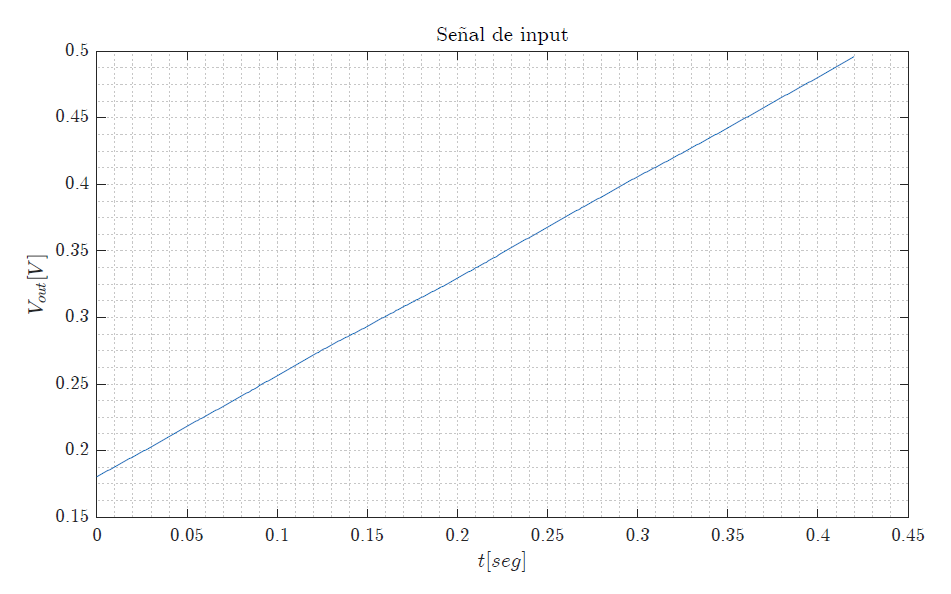
\includegraphics[scale=0.49]{../parte6/Informe/resources/grafica_input_medicion.png}
\caption{Señal de entrada que simulo la salida del integrado LM35}
\label{6_input}
\end{figure}

La Figura \ref{6_input} muestra la señal de entrada implementada para observar el comportamiento de la señal de salida. En la Figura \ref{6_output} se muestra una gráfica con los valores de la tensión de salida vs. el valor de tensión de entrada contrastada con la curva correspondiente a la simulación.

\begin{figure}[H]
\centering
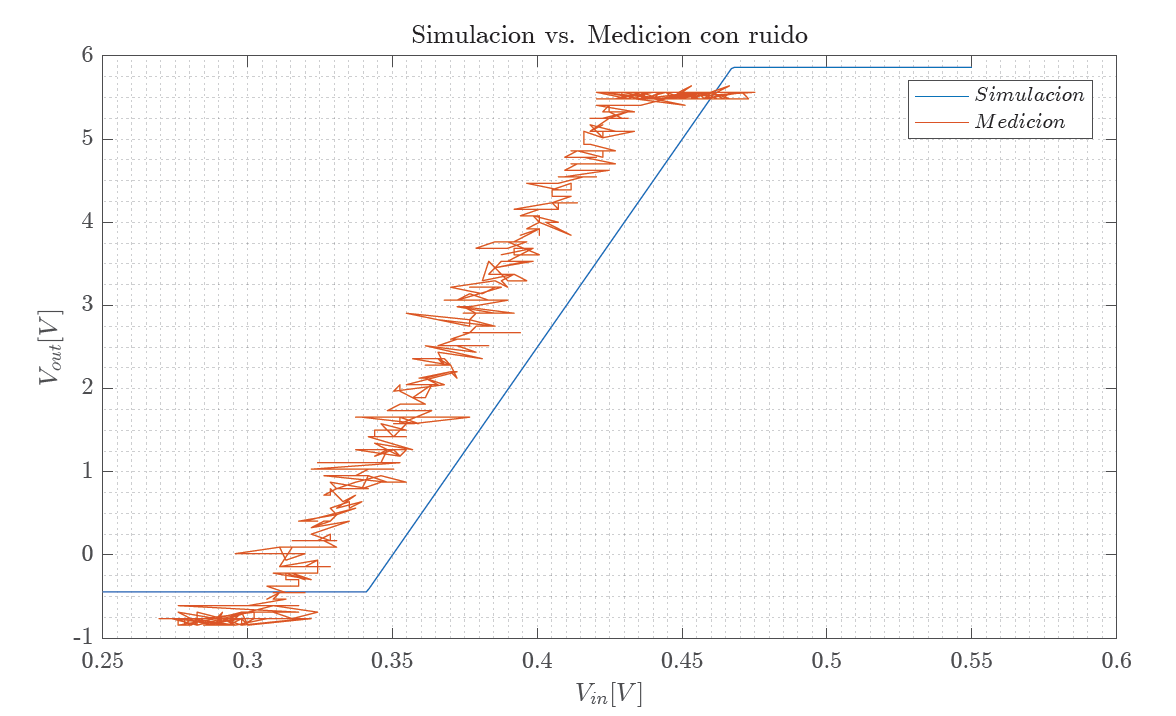
\includegraphics[scale=0.4]{../parte6/Informe/resources/grafica_contraste_ruido.png}
\caption{Tensión de salida vs. tensión de entrada simulada y medida}
\label{6_output}
\end{figure}

\subsubsection{Impedancia de entrada}
Para la medición de la impedancia de entrada se conectó una resistencia en serie a la entrada de la señal del circuito. Se ingresó una señal de entrada constante, y se midió la tensión antes y después de la resistencia mencionada, para así poder calcular la corriente que circula por la misma. Para determinar la impedancia de entrada se calculó el cociente entre la tensión de entrada y la corriente de entrada. 
Con los siguientes datos:

\[V_{in} = 373,44mV\]
\[I_{in} = 256.84\mu A\]

\[R_{in} = \frac{V_{in}}{I_{in}} = 1.45k\Omega\]


\section{Hoja de datos}
La Tabla muestra los datos relevantes al usuario del circuito implementado.

\begin{center}
\begin{tabular}{|c|c|c|}
\hline 
Parámetro & Valor & Unidad \\ 
\hline 
Alimentación ($V_{cc}$) & $\pm 15$ & V \\ 
\hline 
Tensión de salida($V_{out}$) & -0,75 a 5,50 & V \\ 
\hline 
Rango de temperaturas($\Delta T$) & 35 a 45 & $^\circ C$ \\ 
\hline 
Impedancia de entrada($R_{in}$) & 1,45 & $k\Omega$ \\ 
\hline 
\end{tabular} 
\end{center}
